\documentclass{ctexart}
\usepackage{amsmath,bm}
\usepackage{setspace}
\usepackage{xeCJK}
\usepackage{indentfirst}
\usepackage{listings}
\usepackage{graphicx}
\usepackage{subfigure}
\usepackage{amsfonts,amssymb}
\usepackage[a4paper,scale=0.8]{geometry}
\usepackage{hyperref}
\usepackage{pythonhighlight}
\usepackage{float}
\definecolor{mygreen}{rgb}{0,0.6,0}
\definecolor{mygray}{rgb}{0.5,0.5,0.5}
\definecolor{mymauve}{rgb}{0.58,0,0.82}
\lstset{ %
backgroundcolor=\color{white},   % choose the background color
basicstyle=\footnotesize\ttfamily,        % size of fonts used for the code
columns=fullflexible,
breaklines=true,                 % automatic line breaking only at whitespace
captionpos=b,                    % sets the caption-position to bottom
tabsize=4,
commentstyle=\color{mygreen},    % comment style
escapeinside={\%*}{*)},          % if you want to add LaTeX within your code
keywordstyle=\color{blue},       % keyword style
stringstyle=\color{mymauve}\ttfamily,     % string literal style
frame=single,
rulesepcolor=\color{red!20!green!20!blue!20},
% identifierstyle=\color{red},
language=c++,
}
\setCJKmainfont{华光书宋_CNKI}
\newCJKfontfamily\kaiti{华光楷体_CNKI}
\newCJKfontfamily\hei{华光黑体_CNKI}
\newCJKfontfamily\fsong{华光仿宋_CNKI}
\newfontfamily\code{Courier New}
\linespread{1.5} \setlength\parindent{2 em}
\title{\Huge 中国科学技术大学计算机学院\\《计算机图形学理论和应用》实验报告}
\date{\LARGE 2021.07.15}
\begin{document}
\begin{hei}  \maketitle\end{hei}
\begin{figure}[htbp]
    \centering
    
\includegraphics[scale=0.4]{USTC.png}

\end{figure}
\begin{LARGE}\begin{align*} & \text{实验题目:\underline{人脸动画表情系统}} \\
         & \text{学生姓名:\underline{胡毅翔}}                 \\
         & \text{学生学号:\underline{PB18000290}}\end{align*}\end{LARGE}
\par
\par\par
\centerline{\large 计算机实验教学中心制}
\par \centerline {\large 2019年9月}
\newpage
\tableofcontents
\newpage
\section{\hei 实验目的}
\begin{enumerate}
    \item 实现简单的人脸模型;
    \item 实现人脸的表情动画;
    \item 优化人脸动画的流畅性和自然性。
\end{enumerate}
\section{\hei 实验环境}
\begin{enumerate}
    \item PC一台;
    \item Windows 10操作系统;
    \item g++ (Ubuntu 7.5.0-3ubuntu1~18.04) 7.5.0;
    \item Linux version 4.4.0-19041-Microsoft(WSL)。
\end{enumerate}

\section{\hei 人脸模型}
本次实验使用的人脸模型是从www.blender.org下载的.obj文件,其中包含了大量的点和面的信息,对应一个多边形模型,以生成一个相对真实的人脸。而对应的\_KP.obj文件中,则包含了对应人脸模型的关键点信息,用于动画时的控制。
\section{\hei 动画系统}
本次实验的核心代码在于根据关键点(Key Points)的变化,更新其他点,以达成动画的效果。关键点(KP)类的定义如下:
\begin{lstlisting}
class KP {
public:
  // keypoint ID (also reported in the vertex)
  char *id;
  // initial coordinates
  Point location;
  //  index of the mesh
  int indMesh;
  //  index of vertex
  int indVertex;
  // current translation
  Vector translation;

  KP( void ) {
    id = new char[STRINGSIZE];
    location.init();
    indMesh = -1;
    indVertex = -1;
    translation.init();
  }
  ~KP( void ) {
    delete [] id;
  }
};    
\end{lstlisting}
\par main函数结构如下:
\begin{lstlisting}
int main(int argc, char **argv)
{
  if (argc >= 2)
  {
    strcpy(MeshFileName, argv[1]);
  }
  else
  {
    printf("Mesh file (head_modified.obj):");
    fflush(stdin);
    fgets(MeshFileName, STRINGSIZE, stdin);
    if (*MeshFileName == '\n')
    {
      strcpy(MeshFileName, "head_modified.obj");
      ;
    }
    else
    {
      MeshFileName[strlen(MeshFileName) - 1] = 0;
    }
  }
  strcpy(KPFileName, MeshFileName);
  ;
  KPFileName[strlen(KPFileName) - 4] = 0;
  strcat(KPFileName, "_KP.obj");

  printf("Mesh file (%s)\n", MeshFileName);
  printf("KP file (%s)\n", KPFileName);

  // GLUT initialization
  glutInit(&argc, argv);
  glutInitDisplayMode(GLUT_RGBA | GLUT_DOUBLE | GLUT_DEPTH);

  // window intialization
  glutInitWindowSize(WINDOW_WIDTH, WINDOW_HEIGHT);
  glutInitWindowPosition(0, 0);
  glutCreateWindow("Meshes");

  // OpenGL and scene initialization
  initGL();
  init_scene();

  // GLUT callbacks
  // for drawing
  glutDisplayFunc(&window_display);
  // for window resize
  glutReshapeFunc(&window_reshape);
  // for keyboard events
  glutKeyboardFunc(&window_key);
  // for mouse clicks
  glutMouseFunc(&window_mouseFunc);
  // for mouse drags
  glutMotionFunc(&window_motionFunc);
  // for special keys

  // use idle func to run facial animation
  glutIdleFunc(idle_func);

  // main event loop
  glutMainLoop();

  return 1;
}    
\end{lstlisting}
\par 距离权重函数代码如下:
\begin{lstlisting}
// a keypoint weighting scheme: linear weighting
float linear_weight(float distance, float radius, int exponent)
{
  if (distance < radius)
  {
    return 1.0 - distance / radius;
  }
  else
  {
    return 0.f;
  }
}

// a keypoint weighting scheme: the distance's inverse(before normalization)
float inverse_distance_weight(float distance, float radius, int exponent)
{
  if (distance < radius)
  {
    return 1 / distance;
  }
  else
  {
    return 0.f;
  }
}    
\end{lstlisting}
\par 动画函数如下:
\begin{lstlisting}
// moves each vertex according to the translation
// of the keypoints to which this vertex is attached

void animate_vertices_in_mesh(void)
{
  int indKP;
  Vertex *ptVertex = TabVertices;

  for (int indVertex = 0; indVertex < NbVertices;
       (ptVertex++, indVertex++))
  {
    if (ptVertex->weighted == false)
    {
      continue;
    }
    ptVertex->curLocation = ptVertex->location;
    for (int i = 0; i < MAXKPWEIGHTS; i++)
    {
      // TODO
      KP *kp = &TabKPs[ptVertex->indKP[i]];
      ptVertex->curLocation.x += ptVertex->wKP[i] * kp->translation.x;
      ptVertex->curLocation.y += ptVertex->wKP[i] * kp->translation.y;
      ptVertex->curLocation.z += ptVertex->wKP[i] * kp->translation.z;
    }
  }
}    
\end{lstlisting}
\par 缓动函数代码如下:
\begin{lstlisting}
float curve_ease_inout_quad(float elapsed, float duration, float startVal, float endVal)
{
  float u = elapsed / (duration / 2);
  if (u < 1)
  {
    return startVal + (endVal - startVal) / 2 * u * u;
  }
  else
  {
    u--;
    return startVal - (endVal - startVal) / 2 * (u * (u - 2) - 1);
  }
};

float curve_linear(float elapsed, float duration, float startVal, float endVal)
{
  float percent = elapsed / duration;
  return startVal + (endVal - startVal) * percent;
}    
\end{lstlisting}
\section{\hei 运行演示}
\begin{enumerate}
    \item 在主目录(Makefile所在目录)下,执行$make KP-anim-modele$;
    \item 在WSL(Windows Subsystem for Linux)下运行前,需先启动$Xming$,执行$export DISPLAY=:0$,用于显示运行结果;
    \item 执行$./KP-anim-modele$,运行编译生成的文件(在Linux(包括WSL)或Mac OSX上运行);
    \item 输入使用的人脸模型,已提供的有$head_modified_highpoly.obj$,$head_modified.obj$;
    \item 加载人脸模型,出现动画界面;
    \item 点击鼠标左键拖拽,旋转人脸模型;
    \item 输入'<'或'>',缩小或放大模型;
    \item 输入'1'-'8',运行表情系统,分别对应的表情为:中性,开心,失落,惊讶,愤怒,厌恶,恐惧,默认;
    \item 输入'+'或'-',加快或放慢动画速度;
    \item 输入'q'或'w',选择二次缓动函数或线性缓动函数;
    \item 输入'a'或's',选择反距离权重或线性权重。
\end{enumerate}
运行结果截图如下:
\begin{figure}[htbp]
    \centering
    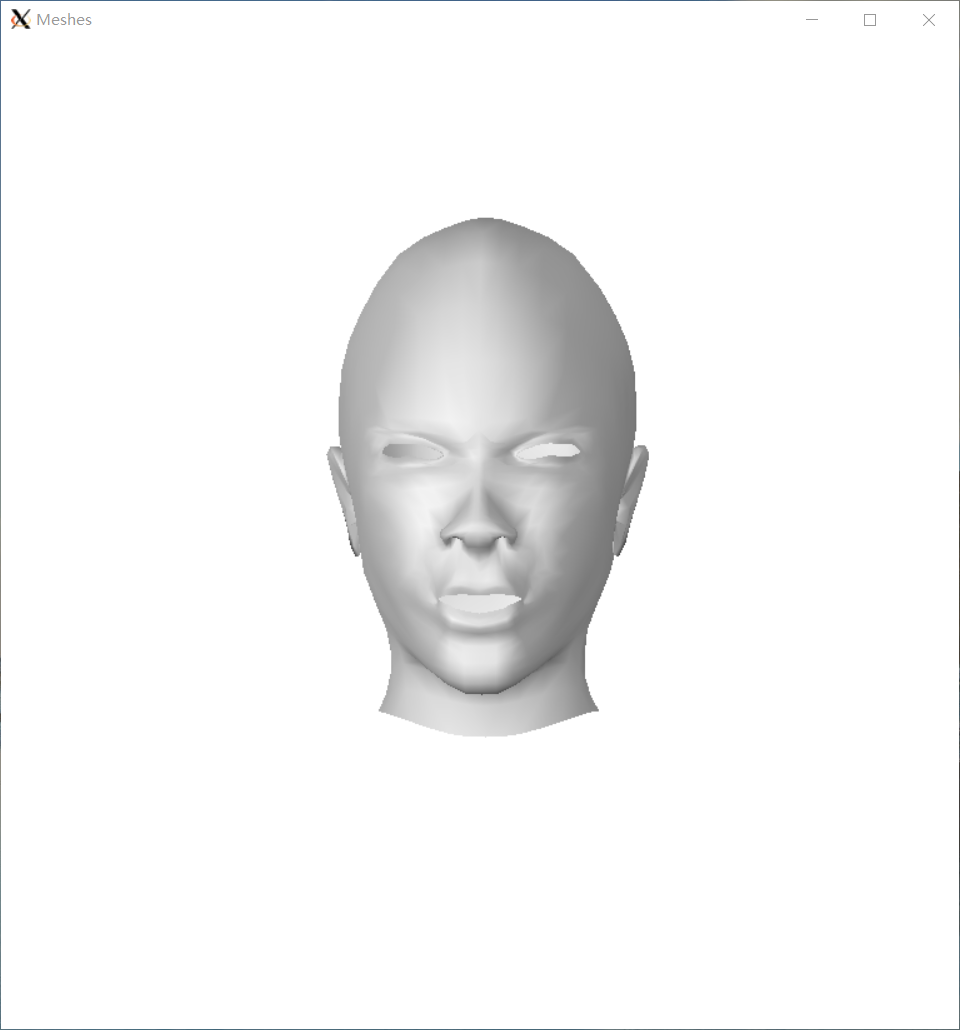
\includegraphics[scale=0.5]{mesh.png}

\end{figure}
\par 完整演示视频链接\href{https://www.bilibili.com/video/BV1Tq4y1s7u8}{点击此处}。
\end{document}